\documentclass[a4paper, UTF8, 12pt]{article}

\usepackage{ctex}
\usepackage{abstract}
\usepackage{geometry}
\usepackage{graphicx}
\usepackage{float}
\usepackage{caption}
\usepackage{enumerate}
\usepackage{natbib}
\usepackage{amsmath}

\usepackage{hyperref}
\hypersetup{
    colorlinks=true,   % false, ,链接黑色, 外有红框
    linkcolor=black, % 目录颜色, 脚注颜色
    filecolor=blue, % 链接本地文件的链接颜色
    urlcolor=cyan, % 网页链接颜色
    anchorcolor=blue,
    citecolor=green    % 参考文献颜色
}
\graphicspath{{pics/}}
\renewcommand{\theequation}{\arabic{section}.\arabic{equation}}

\bibliographystyle{plainnat}

\begin{document}
\title{\Huge 工程测量-平面拟合及可视化}
\author{\Large 
        1931991 任家平 \\[12pt]
        同济大学 \\[12pt]
        测绘与地理信息学院}
\date{2020-06-04}
\maketitle
\thispagestyle{empty}

\renewcommand\abstractname{\Large\textbf{摘要}}
\begin{abstract}
    \center{
    \parbox[s]{14cm}{ 
    
    \qquad 记录使用\href{https://github.com/RaoUmer/SRResCGAN}{srrescgan}模型训练遥感影像超分结果.
    
    }}
\end{abstract}

\addcontentsline{toc}{section}{摘要}
\pagenumbering{roman}

\newpage
\pagenumbering{Roman}
\tableofcontents

\newpage
\pagenumbering{arabic}

本周主要在配置环境做实验, 因此报告内容并不丰满. 主要任务是对超分和影像翻译进行深度学习环境进行配置. 对于超分思路为: 

\begin{enumerate}
    \item 使用常规超分数据集跑通训练代码 
    \item 使用自己的数据根据要求制作训练数据集
\end{enumerate}

其中超分尝试了以下三个模型, 流程还未跑通. 

\begin{itemize}
    \item \href{https://github.com/LoSealL/VideoSuperResolution}{LoSealL/VideoSuperResolution} 该代码为总结近年来的超分模型.
    \item \href{https://github.com/hejingwenhejingwen/AdaFM}{hejingwenhejingwen/AdaFM} 2019年提出的超分模型
    \item \href{https://github.com/sanghyun-son/EDSR-PyTorch}{sanghyun-son/EDSR-PyTorch} 尝试中.
\end{itemize}

对于影像翻译深度学习模型, 继承已有的代码, 跑通训练流程所遇到问题比超分少.

现在结果: 已经跑通pix2pix模型, 大致了解训练测试参数的调整, 模型更改, 损失函数更改等. 具体细节还需要进一步学习. 整理数据集, 现已有三个数据集, WHU, OPT2SAR, OPT2SAR\_dong. 对于数据集制作(实验角度), 其关键在于不同源影像的配准, 与配准后的自动化裁剪. 另外要注意的一点是sar影像的处理方式, 是像WHU处理为伪彩色影像进行翻译, 还是直接用预处理后的影像进行翻译. 

下周计划:
\begin{itemize}
    \item 学习GAN网络基础知识, Generator, Discriminator
    \item 跑通超分流程
\end{itemize}

还需要制作超分数据集自动化制作工具






\section{Sentinel-1卫星产品参数分析}
\section{SRResCGAN实验}

\begin{frame}{训练结果}
    第一次训练, $lr_{G}=0.0001, lr_{D}=0.0003$最终的D\_fake\_output和D\_real\_output一直相差较大, 说明判别器远强于生成器; 增大生成器学习率$lr_{G}=0.001$, 依然如此. 除学习率外, 可调整参数有网络结构, 各种损失函数的权重和类型. 
\end{frame}

\begin{frame}{PNSR SSIM}
    \footnotesize
    \begin{tabular}{l|p{3cm}|p{3cm}}
        \hline
                 & PNSR & SSIM     \\ \hline
        01Bicubic & 17.89dB & 0.3750 \\ \hline
        01SRResCGAN & 19.45dB & 0.4412 \\ \hline
        02BIcubic &  19.48dB & 0.4240 \\ \hline
        02SRResCGAN & 21.34dB & 0.4930 \\ \hline
        03BIcubic &  23.83dB & 0.6836 \\ \hline
        03SRResCGAN & 24.30dB & 0.6845 \\ \hline
        04BIcubic &  18.54dB & 0.3384 \\ \hline
        04SRResCGAN & 19.15dB & 0.3536 \\ \hline
        05BIcubic &  21.42dB & 0.4730 \\ \hline
        05SRResCGAN & 22.56dB & 0.4893 \\ \hline
    \end{tabular}

    一方面没有训练好; 一方面本身影像对存在一定差异
\end{frame}

\begin{frame}{细节对比}
    \begin{figure}[!htbp]
        \centering
        \subfloat[gt]{\label{fig:0301a}
        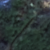
\includegraphics[height=1cm]{pic/pic0301gt.png}}
        \quad
        \subfloat[bic]{\label{fig:0301b}
        
\includegraphics[height=1cm]{pic/pic0301bic.png}}
        \quad
        \subfloat[sr]{\label{fig:0301c}
        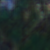
\includegraphics[height=1cm]{pic/pic0301sr.png}}
        \caption{细部对比01}
        \label{fig:0301}
    \end{figure}

    \begin{figure}[!htbp]
        \centering
        \subfloat[gt]{\label{fig:0302a}
        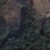
\includegraphics[height=1cm]{pic/pic0302gt.png}}
        \quad
        \subfloat[bic]{\label{fig:0302b}
        
\includegraphics[height=1cm]{pic/pic0302bic.png}}
        \quad
        \subfloat[sr]{\label{fig:0302c}
        
\includegraphics[height=1cm]{pic/pic0302sr.png}}
        \caption{细部对比02}
        \label{fig:0302}
    \end{figure}

    
\end{frame}

\begin{frame}{细节对比}
    \begin{figure}[!htbp]
        \centering
        \subfloat[gt]{\label{fig:0303a}
        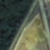
\includegraphics[height=1cm]{pic/pic0303gt.png}}
        \quad
        \subfloat[bic]{\label{fig:0303b}
        
\includegraphics[height=1cm]{pic/pic0303bic.png}}
        \quad
        \subfloat[sr]{\label{fig:0303c}
        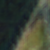
\includegraphics[height=1cm]{pic/pic0303sr.png}}
        \caption{细部对比03}
        \label{fig:0303}
    \end{figure}

    \begin{figure}[!htbp]
        \centering
        \subfloat[gt]{\label{fig:0304a}
        
\includegraphics[height=1cm]{pic/pic0304gt.png}}
        \quad
        \subfloat[bic]{\label{fig:0304b}
        
\includegraphics[height=1cm]{pic/pic0304bic.png}}
        \quad
        \subfloat[sr]{\label{fig:0304c}
        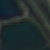
\includegraphics[height=1cm]{pic/pic0304sr.png}}
        \caption{细部对比04}
        \label{fig:0304}
    \end{figure}
\end{frame}

\begin{frame}{细节对比}
    \begin{figure}[!htbp]
        \centering
        \subfloat[gt]{\label{fig:0305a}
        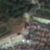
\includegraphics[height=1cm]{pic/pic0305gt.png}}
        \quad
        \subfloat[bic]{\label{fig:0305b}
        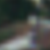
\includegraphics[height=1cm]{pic/pic0305bic.png}}
        \quad
        \subfloat[sr]{\label{fig:0305c}
        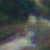
\includegraphics[height=1cm]{pic/pic0305sr.png}}
        \caption{细部对比05}
        \label{fig:0305}
    \end{figure}

    \begin{figure}[!htbp]
        \centering
        \subfloat[gt]{\label{fig:0306a}
        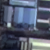
\includegraphics[height=1cm]{pic/pic0306gt.png}}
        \quad
        \subfloat[bic]{\label{fig:0306b}
        
\includegraphics[height=1cm]{pic/pic0306bic.png}}
        \quad
        \subfloat[sr]{\label{fig:0306c}
        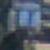
\includegraphics[height=1cm]{pic/pic0306sr.png}}
        \caption{细部对比06}
        \label{fig:0306}
    \end{figure}
\end{frame}
\section{Time Series Classification from Scratch with Deep Neural Networks: A Strong Baseline}

\paragraph*{para---para
    \textcolor[RGB]{17, 205, 29}{}}
\begin{quotation}
    \itshape

\end{quotation}

\paragraph*{para---para
    \textcolor[RGB]{17, 205, 29}{}}
\begin{quotation}
    \itshape

\end{quotation}

\paragraph*{para---para
    \textcolor[RGB]{17, 205, 29}{}}
\begin{quotation}
    \itshape

\end{quotation}

\paragraph*{para---para
    \textcolor[RGB]{17, 205, 29}{}}
\begin{quotation}
    \itshape

\end{quotation}

\paragraph*{para---para
    \textcolor[RGB]{17, 205, 29}{}}
\begin{quotation}
    \itshape

\end{quotation}

\listoffigures
\addcontentsline{toc}{section}{插图目录}
\listoftables
\addcontentsline{toc}{section}{表格目录}
\newpage
\nocite{*}

\bibliography{ref}
\addcontentsline{toc}{section}{参考文献}

\end{document}